\documentclass{report}
\usepackage{amsmath}
\usepackage{amssymb}
\usepackage{xeCJK}
\usepackage{hyperref}
\usepackage{graphicx}
\usepackage{listings}
\setCJKmainfont{STKaiti}
\begin{document}
\chapter{线性回归}
\section{摘要}
你好,我是生而为弟。\\
在学习NLP的过程中,我对于公式的推导完全不会,因此我决定从头学习机器学习的理论推导。\\
本期主要分为两个部分:
\begin{itemize}
	\item[] 第一部分将从矩阵,几何,概率三个视角,对线性回归-最小二乘法的闭式解进行推导,并提供参考代码。
	\item[] 第二部分将从矩阵和概率两个视角,对带正则化的最小二乘法的闭式解进行推导,并构造一个完整的线性回归类,同时实现闭式解求法与梯度下降解法。
\end{itemize}
\section{介绍}
线性回归模型是利用线性函数对一个或多个自变量和因变量($y$)之间关系进行拟合的模型。\\
目标变量($y$)为连续数值型 ,如:房价,人数,降雨量 回归模型是寻找一个输入变量到输出变量之间的映射函数。\\
回归问题的学习等价于函数拟合:使用一条函数曲线使其很好的拟合已知数据且能够预测未知数据。\\
回归问题分为模型的学习和预测两个过程。基于给定的训练数据集构建一个模型,根据新的输入数据预测相应的输出。
\section{不带正则化的算法}
\subsection{矩阵视角}
注:一般情况下,我们讨论的向量都是列向量,因此推导过程中为保证矩阵的形状,会大量使用转置符\\
已知数据集$D=\{(x_1,y_1),(x_2,y_2)...(x_n,y_n)\}$\\
其中$x_i\in R^p,y_i\in R,i=1,2,...,n$\\
$$
X=(x_1,x_2,...,x_n)^T=\begin{pmatrix}
x_{11}&x_{12}&...&X_{1p}\\
x_{21}&x_{22}&...&x_{2p}\\
.&.&.&.&\\
.&.&.&.&\\
.&.&.&.&\\
x_{n1}&x_{n2}&...&x_{np}\\
\end{pmatrix}_{np}
$$
$$
Y=(y1,y2,...,y_n)_{n1}^T
$$
这是我们建立的模型:$f(w)=w^Tx+w_0x_0。$\\
一般令$x_0=1$,而$b=w_0x_0$,$b$是偏置(bias),$w$为权重(weight),下面为了推导的方便,我们将$w_0$并入$w$中,$x_0$并入$X$中\\
因此模型更为$f(w)=w^Tx$
最小二乘法的损失函数为:
$$
L(w)=\sum_{i=1}^{i=n}\|y_i-w^T x_i\|_2^2
$$
$$
=\begin{pmatrix}
y_1-w^Tx_1&y_2-w^Tx_2&...&y_n-w^Tx_n
\end{pmatrix}
\begin{pmatrix}
y_1-w^Tx_1\\
y_2-w^Tx_2\\
.\\
.\\
.\\
y_n-w^Tx_n\\
\end{pmatrix}
$$
$$
=(Y^T-w^TX^T)(Y^T-w^TX^T)^T
$$
$$
=(Y^T-w^TX^T)(Y-Xw)
$$
$$
=Y^TY-w^TX^TY-Y^TXw+w^TX^TXw
$$
仔细观察发现第二三项是互相转置的,而观察它的矩阵形状: $(1,p)(p,n)(n,1)=(1,1)$\\
得知这两项为标量,而标量的转置还是本身,因此可将两项合并,得
$$
L(w)=Y^TY-2w^TX^TY+w^TX^TXw
$$
因此$\hat{w}=argmin(L(w))$
下面要求出$L(w)$的最小值,对$L(w)$求导\\
可以看到式子共三项,第一项与$w$无关,可以去掉。那么剩余两项就要涉及到矩阵求导了\\
关于矩阵求导,笔者推荐一位博主的三篇文章(比教科书还详细,严谨,每个公式都有证明)
\begin{itemize}
	\item \href{https://zhuanlan.zhihu.com/p/263777564}{矩阵求导——本质篇}
	\item \href{https://zhuanlan.zhihu.com/p/273729929}{矩阵求导——基础篇}
	\item \href{https://zhuanlan.zhihu.com/p/288541909}{矩阵求导——进阶篇}
\end{itemize}
下面为上述两项的导数求解过程:\\
因为$X,Y$为常数矩阵,因此可直接求出导数,但因为是对$w$求导,因此要对结果进行转置
$$
\frac{d(2w^TX^TY)}{dw}=2X^TY
$$
下面求解第三项
$$
d(w^TX^TXw)=tr(d(w^TX^TXw))=tr(X^TXd(w^Tw))
$$
$$
=tr(X^TX(d(w^T)w+w^Td(w)))=tr(X^TXw(dw)^T)+tr(X^TXw^Tdw)
$$
$$
=tr(w^TX^TXdw)+tr(X^TXw^Tdw)=tr(2X^TXw^Tdw)
$$
所以
$$
\frac{d(w^TX^TXw)}{dw}=2wX^TX
$$
所以$\frac{dL(w)}{dw}=2X^TXw-2X^TY$\\
令导数等于0,得出最小二乘的闭式解:
$$
\hat{w}=(X^TX)^{-1}X^TY
$$
\subsection{几何视角}
$$
X=(x_1,x_2,...,x_n)^T=\begin{pmatrix}
x_{11}&x_{12}&...&X_{1p}\\
x_{21}&x_{22}&...&x_{2p}\\
.&.&.&.&\\
.&.&.&.&\\
.&.&.&.&\\
x_{n1}&x_{n2}&...&x_{np}\\
\end{pmatrix}_{np}
$$
$$
Y=(y1,y2,...,y_n)_{n1}^T
$$
在几何视角下,我们将$X$看作是一个$p$维的向量\\
$X$的第一维是$(x_{11},x_{21},...,x_{n1})$,$X$的第$p$维是$(x_{1p},x_{2p},...,x_{np})$
而这里的$Y$被看作是一个一维的向量\\
现在我们假设$p=2$,因为比较好画。示意图如下(俺真的画了好久,观众老爷们给波三连吧)\\\\
\begin{figure}
\center
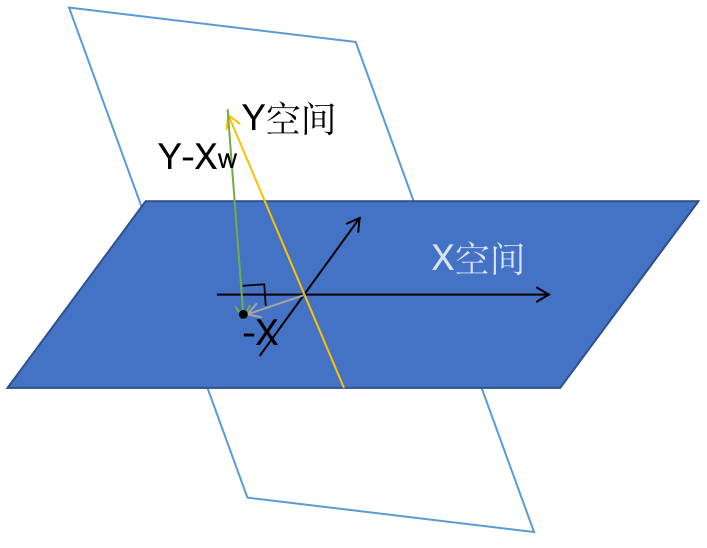
\includegraphics[width = 0.7 \textwidth]{/Users/btobab/TeX-Projects/figures/1}
\end{figure}
将模型改为$f(w)=Xw$,意为对$X$向量施以$w$权重的放缩\\
而最小二乘的几何意义就是找到一个$w$,使得$Y-Xw$这个向量到$X$空间的距离最小,那最小的情况当然就是与$X$空间垂直\\
所以我们有式子$X^T(Y-Xw)=0$\\
从而求解$w$:
$$
X^TXw=X^TY
$$
$$
\hat{w}=(X^TX)^{-1}X^TY
$$
可以看到求出的$w$与矩阵视角的结果相同。
\subsection{概率视角}
首先明确,现实中是很难用一条直线去拟合分布的。真实的数据必然存在一定的随机性,也就是噪声。\\
因此我们假设噪声$\epsilon\backsim N(0,\sigma^2)$\\
所以$y=f(w)+\epsilon=w^Tx+\epsilon$\\
所以$y|x;w\backsim N(w^Tx,\sigma^2)$\\
带入高斯分布的概率密度函数:
$$
p(y|x;w)=\frac{1}{\sqrt{2\pi}\sigma}e^{-\frac{(y-w^Tx)^2}{2\sigma^2}}
$$
下面使用 MLE (极大似然估计):\\
注:所谓极大似然估计,即通过大量的采样得到相对频率,去逼近概率\\
我们设一个函数$\mathcal{L}(w)=\log{p(Y|X;w)}$\\
因为$n$个数据之间是独立的,因此可以将概率改为连乘的形式。\\
$\mathcal{L}(w)=\log{\Pi_{i=1}^np(y_i|x_i;w)}=\Sigma_{i=1}^n \log{p(y_i|x_i;w)}$\\
将高斯分布的概率密度函数带入式子:\\
$\mathcal{L}(w)=\Sigma_{i=1}^n(\log{\frac{1}{\sqrt{2\pi}\sigma}}-\frac{(y-w^Tx)^2}{2\sigma^2})$\\
因为前一项与$w$无关,所以可以忽略\\
所以:
$$
\begin{aligned}
\hat{w}
&=argmax \mathcal{L}(w)\\
&=argmax \Sigma_{i=1}^n -\frac{(y-w^Tx)^2}{2\sigma^2}\\
&=argmin \Sigma_{i=1}^n (y-w^Tx)^2
\end{aligned}
$$
而使用极大似然估计得到的结论正是最小二乘法的定义。\\
这也恰好说明,最小二乘法隐藏着一个噪声为高斯分布的假设。
\section{不带正则项的实作}
\begin{lstlisting}[language={python}]
%matplotlib inline
import numpy as np
import matplotlib.pyplot as plt

# 样本数
n = 1000
# 噪声
epsilon = 1
X = np.expand_dims(np.linspace(0,100,1000), axis=-1)
w = np.asarray([5.2])
Y = X  w
# 增加噪声扰动
X += np.random.normal(scale=epsilon, size=(X.shape))
X_T = X.transpose()
w_hat = np.matmul(np.linalg.pinv((np.matmul(X_T, X))), np.matmul(X_T, Y))
print(w_hat)
plt.scatter(X, Y, s=3, c="y")
Y_hat = X  w_hat
plt.plot(X, Y_hat)
plt.show()
\end{lstlisting}
\section{带正则化的算法}
\subsection{矩阵视角}
首先给出带正则项的新损失函数:
$$
\mathcal{L}(w)=\Sigma_{i=1}^{n}||y_i-w^T  x_i||^2 + \lambda  ||w||^2
$$
然后引用不带正则化的矩阵视角的损失函数的推导形式:
$$
\mathcal{L}(w)=Y^TY-2w^TX^TY+w^TX^TX w+\lambda  ||w||^2
$$
所以$\hat{w}=argmax(\mathcal{L}(w))$\\
对$\mathcal{L}(w)$求导,得到:
$$
\frac{\partial \mathcal{L}(w)}{\partial w}=2X^TXw-2X^T Y+2\lambda  w 
$$
令导数为0,得到带正则化的最小二乘法的闭式解:
$$
\hat{w}=(X^TX+\lambda  I)^{-1} X^TY
$$
$I$为单位矩阵
\subsection{概率视角}
假设噪声$\epsilon \backsim N(0,\sigma_1^2) \ w \backsim N(0,\sigma_2^2)$\\
因为$y=w^T x + \epsilon$\\
所以$y|w \backsim N(w^T x,\sigma_1^2)$
下面我们使用 MAP(最大后验估计):
由贝叶斯定理得:
$$
P(w|Y)=\frac{P(Y|w) P(w)}{P(Y)}
$$
其中$P(w)$为先验概率,$P(Y|w)$为似然概率,$P(Y)$为归一化概率,先验概率乘似然概率并归一化得到后验概率$P(w|Y)$
其中$P(Y)$实际上为常数,因此:
$$
\hat{w}=argmax(P(w|Y))=argmax(P(Y|w) P(w))=argmax(log(P(Y|w) P(w)))
$$
因为每个样本间是独立的,因此可以将概率连乘
$$
=argmax(log(\prod_{i=1}^n P(y_i|w) P(w)))=argmax(\sum_{i=1}^n log(P(y_i|w)+ log(P(w))))
$$
带入高斯分布的概率密度函数,得到:
$$
\hat{w}=argmax(\sum_{i=1}^nlog(\frac{1}{\sqrt{2\pi} \sigma_1})-\frac{(y_i-w^T x_i)^2}{2\sigma_1^2}+log(\frac{1}{\sqrt{2 \pi} \sigma_2})-\frac{w^2}{2\sigma_2^2})
$$
因为$\sigma_1,\sigma_2$都为超参数,因此可以省略\\
所以:
$$
\hat{w}=argmin(\sum_{i=1}^n \frac{(y_i-w^T x_i)^2}{2\sigma_1^2}+\frac{w^2}{2\sigma_2^2})
$$
$$
=argmin(\sum_{i=1}^n (y_i-w^T x_i)^2+\frac{\sigma_1^2}{\sigma_2^2} w^2)
$$
可以看到,使用 MAP 推导出的结果正是带正则项的最小二乘的定义
\newpage
\section{带正则项的实作}
\begin{lstlisting}[language={python}]
import os
os.chdir("../")
import numpy as np
import matplotlib.pyplot as plt
from models.linear_models import LinearRegression

X_ = np.expand_dims(np.linspace(0, 10, 1000), axis=-1)
X = np.c_[X_, np.ones(1000)]
w = np.asarray([5.2, 1])
Y = X.dot(w)
X = np.r_[X, np.asarray([[11, 1], [12, 1], [13, 1]])]
Y = np.r_[Y, np.asarray([100, 110, 120])]

model = LinearRegression(l2_ratio=1e1, epoch_num=1000, lr=1e-2, batch_size=100, if_standard=False)
model.fit(X[:, :-1], Y)
print(model.get_params())
model.draw(X[:, :-1], Y)
\end{lstlisting}
\end{document}